%!TEX root = ../master.tex
\chapter{Design}\label{ch:design}
The following chapter contains the designs for Terra Mystica's augmented board's interface and its requirement specification. They are based on the concept idea of the interactive board for Terra Mystica and the lo-fi test of a mock-up version of this concept.

\section{An interactive board for Terra Mystica}
This project aims to create an interactive board for Terra Mystica, using computer vision to detect hand contact on the board via a camera below its surface. With the hand contact, the user should be able to change the colour of the hexagon-shaped tiles in the game. The idea is that the board itself is a projection from below, and the board should change according to inputs on the table's surface.

The interactive board will eliminate the need for terrain game pieces, since it will manage terraforming digitally for the player. It may also streamline other elements of the game.

A possible expansion of the project would be detection of game pieces, which can be used to measure amount of power to be offered after game piece placement.

\section{Lo-fi test}
\begin{figure}
\centering
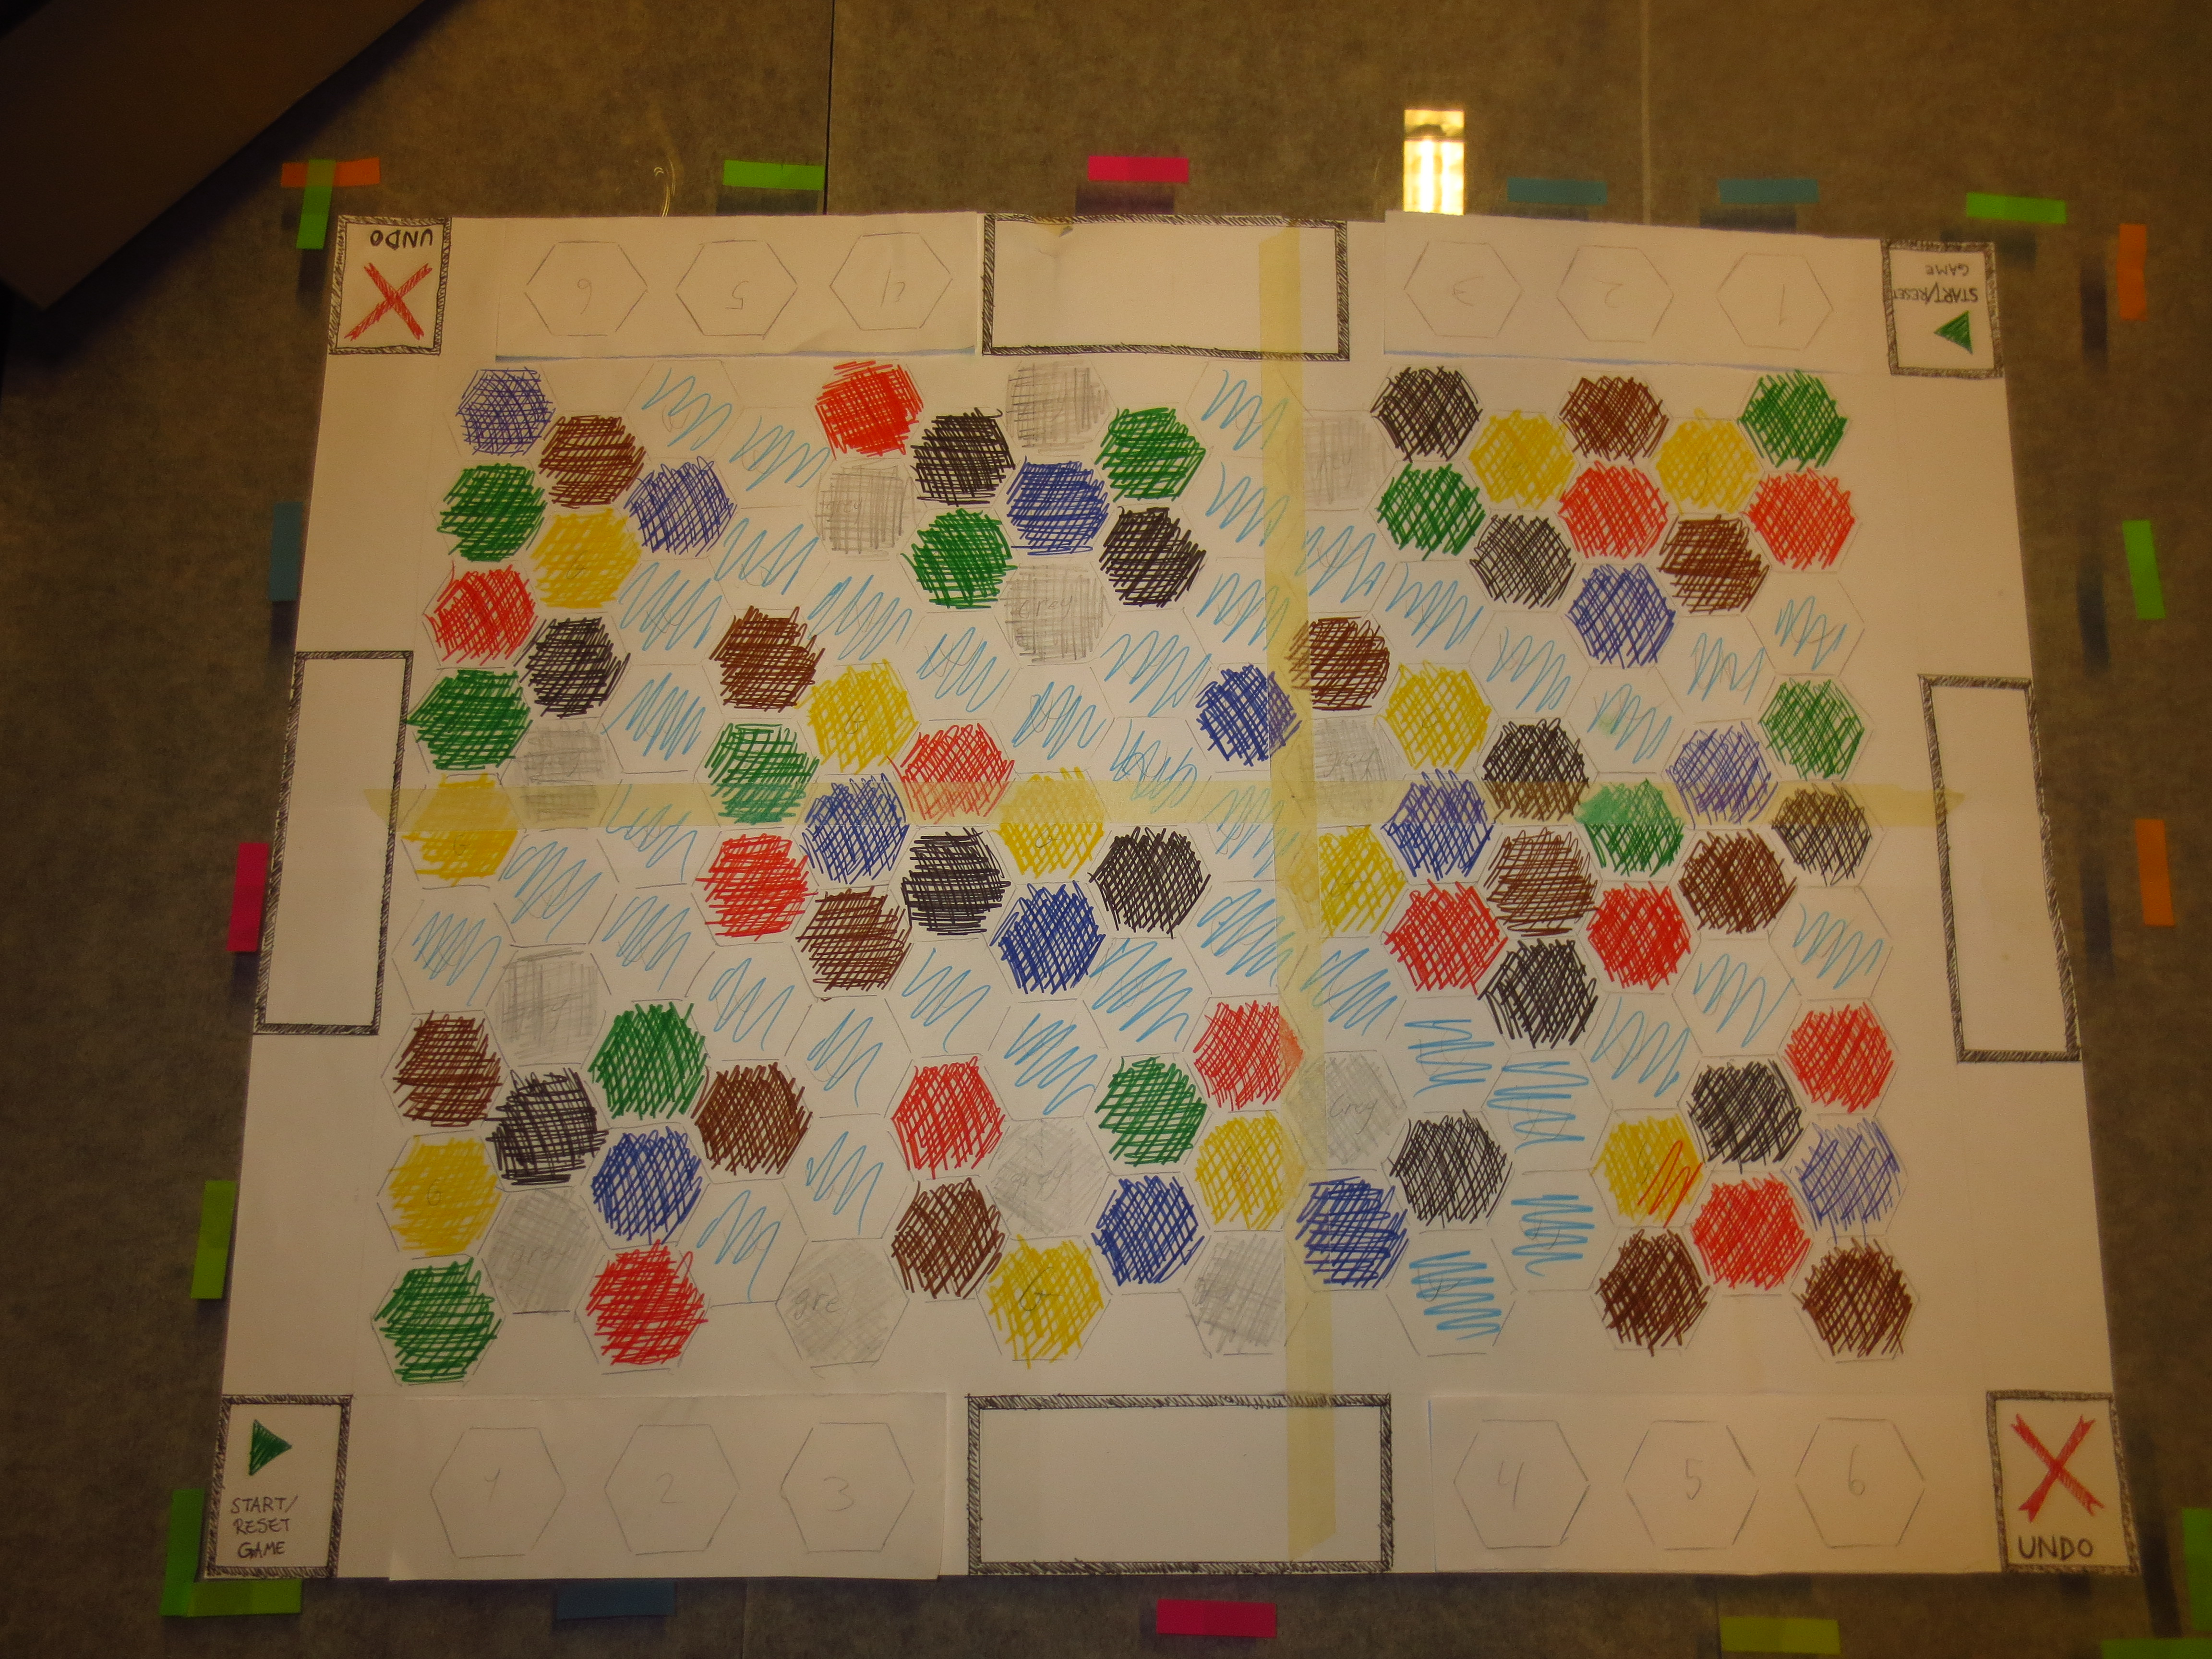
\includegraphics[width=0.9\textwidth]{IMG_0001}
\caption{The Lo-Fi board}
\end{figure}

After defining the initial design, a lo-fi test was conducted to test whether the areas of interest were large enough, the defined gestures were easy to perform, and if the increased size had any effect on the gameplay. We also wanted a first outside opinion of the game without the terraforming pieces.

\subsection{Procedure}
For the lo-fi we had three participants: Two female participants and one male, aged 20-25. 
They were all familiar with the game Terra Mystica, so they did not need to learn the game first. They only played two rounds, since one of the key points of the test was to learn if the gestures and the areas were appropriate. 

The participants were introduced to the Lo-Fi board, by the primary interviewer who also acted as the "program", about how the gestures worked and where they worked. They then played two rounds of the game, with some functions removed since they had no effect when only playing two rounds. During the game they commented out loud, which was noted down by the secondary interviewer who also noted down their reactions and behaviour. 
After the game they were asked some questions in a loosely structured group interview. 
The whole test was filmed.

\subsection{Results} 
The participants all had a little bit of trouble remembering to do the terraforming gesture in the beginning, but they were all pretty sure that with a little more playing it would come naturally. One female participants said: \textit{” I think it comes by itself when you play the game some more.”}. They also mentioned that it might be easier to remember to do the "start of turn"-gesture if the non-interactive areas of the board lit up in the colour of the currently selected player, as another female participant said: \textit{” I think it would help with some light or something like that”}.


They generally liked the bigger board, since this made the hexes and other touch areas bigger, but they did also mention that for short people, it might be a problem to reach the other end of the board. The male participant said: \textit{"I think it is easier with touch control and such, if it was the normal board it would have been a bit harder for me to place my fingers on it"} while one of the female participants said \textit{"It’s just [that] small people aren’t allowed [to stand] at the ends of the table"}.

The participants were curious to why the buildings, their placements and their upgrades were not digital like the terraforming. They then made the guess themselves that reducing the use and amount of game pieces further would remove some of the tangibility they like about the game. They mentioned that the augmented version made terraforming and building seem like very different actions to execute, and a way to make them seem more alike would be to also make touch interactions with the board when you were about to place building pieces.

The personal player input area could be utilised better. Maybe it could indicate income or victory points or just indicate whenever it is your turn. 

The conclusions of the lo-fi test are that the gestures are easy to do and the areas of interest are large enough. The increased size of the board did make it harder for smaller players. The next step is then to discern if the program will be able to recognise the gestures. 

\section{Board interface}\label{sec:BoardInterface}
\begin{figure}
\centering
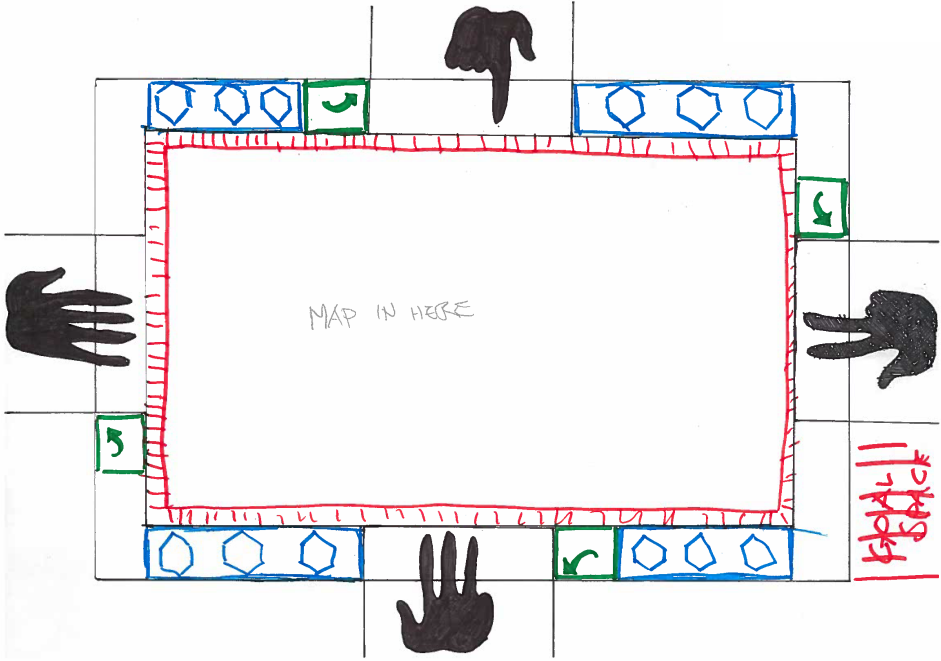
\includegraphics[width=0.9\textwidth]{sketchGUI}
\caption{Sketch illustrating the interface}
\label{fig:sketchGUI}
\end{figure}

The board interface itself should resemble the Terra Mystica Board to some extent, as shown on Figure~\ref{fig:sketchGUI}. The following elements should be on the board in the minimum implementation:
\begin{itemize}
\item A map consisting of hexagonal tiles, varying in colour. By default, they will be arranged like the original game board, but all non-river tiles should be able to change colour.
\item Four areas (marked by the hand icon on Figure~\ref{fig:sketchGUI}), where the players can indicate through gestures that it is their turn.
\item A space showing the global power actions which can only be taken once per round by any player. These are marked on Figure~\ref{fig:sketchGUI} in blue. In the minimum implementation, these are not interactive. However, as a further iteration, they can be made interactive, so that it is visible whether the action has been used or not without using tokens.
\item A victory point counter surrounding the map, shown as a red border on Figure~\ref{fig:sketchGUI}. In the minimum implementation, this is not interactive, and the points each player has accumulated must be shown using tokens, as in the original game. A further iteration to this could be to instead manage the points digitally, either by touching the point border itself, or adding add/subtract buttons at the edge of the board.
\item A space where the global goals for this round can be placed. These are managed using game pieces.
\end{itemize}

The following are not required for the minimum implementation, but can be added if time allows:
\begin{itemize}
\item Some undo buttons, marked on Figure~\ref{fig:sketchGUI} in green. These should be interactive, in case a players makes an incorrect action.
\item Detection of building placement, allowing the program to see when power should be offered to another player. The interface could then indicate that power needs to be offered, and in an ideal implementation, how much power. This would require shape recognition of the game pieces.
\item The empty spaces around the edge of the board could be coloured in the currently selected player's colour. This way, it would be visualised whether a player needs to indicate that it is their turn or not.
\item A space showing information about the players, such as race, colour, points, power, etc.
\item An area to place unused building pieces.
\item A space keeping track of the cult track, showing how many points each player has with the different cults.
\end{itemize}

\section{Requirement specifications}\label{sec:ReqSpec}
The following is the specifications of the usability- and software-based requirements needed in order to to design, build and program the interactive board for Terra Mystica. Note that not all of these are necessary to implement in the minimum implementation version of the product, as seen in this project. \todo{Add a reference here to the relevant section in final product}

\begin{enumerate}
\item On each of the four sides of the board, there needs to be an area where players can place a hand showing 1-4 fingers, indicating which player wishes to take their turn. The program must be able to read whether one, two, three, or four fingers have been placed on one of the player selection areas. The player with the corresponding amount of fingers as their gesture should then be selected.
	\begin{enumerate}
	\item Each of these four players must have a corresponding terrain type, represented by a colour.
	\item This must be successful 90\% of the time, as the type of tile placement depends on the player selected.
	\end{enumerate}
\item In the middle of the board, there should be a map consisting of 112 hexagonal tiles. On a player's turn, the program must be able to detect when a tile is selected for terraforming - that is, when a player places three fingers on the tile in question. This tile must then change to the terrain type of the last player who was selected.
	\begin{enumerate}
	\item This must be successful 90\% of the time. It is crucial that the program can tell the difference between placing a game piece on the board, and having the player select a tile via the three finger input. Depending on the efficiency of the program’s BLOB extraction, this might cause misunderstandings from the program.
	\end{enumerate}
\item In case of misplacement of terraforming, the program must be able to detect the use of an undo-button, which should be done with the same gesture as with the terraforming, but instead of doing the gesture on the map, the gesture is done on a visible button, which will be placed near the border, separate from the map.
	\begin{enumerate}
	\item This must be successful 90\% of the time.
	\item The undo-buttons area of interest needs to be secluded from the other areas of interest, so it can not accidentally be interacted with. 
	\end{enumerate}
\item In the game, there are actions which all players can take, but they can only be taken once per round. In the analogue game, a token is placed on the icon for the action when this happens. For the minimum implementation, this does not need to be managed digitally. However, there should be spaces on the board showing the different actions, on which the players can place tokens in order to remember which actions are already taken. There are six of these actions in total. All of these actions should be represented on the board twice; once on each side of the board, so that they are reachable by all players. This is shown in Figure \ref{fig:sketchGUI}, where the actions are the blue areas. 
	\begin{enumerate}
	\item A further implementation which is optional is to make the actions managed digitally. When an action is used, the player must select the action they wish to use by doing the same gesture as when terraforming. Doing this should toggle the action on and off. When the action is turned off, a cross should appear on the action area, showing the players that the action can now not be used.
	\end{enumerate}
\item The digital board should have a point counter. That is, a border around the board consisting of 100 tiles numbered 1-100. The red border on Figure~\ref{fig:sketchGUI} shows its placement. This border should not be managed digitally, but the players should be able to move a coloured token representing themselves from tile to tile, visualising how many points they have. The program should ignore the tokens placed on this border.
\item The board should have a space where the players can place the game pieces that represent the game goals. This space should not be interactive. This space is represented as the red space to the side on Figure \ref{fig:sketchGUI}. These are goals that either apply to only a single round, or to a whole game. Just as with the point counter, the goals should not be managed digitally, but just be covered with game pieces when they are not important.
	\begin{enumerate}
	\item Another optional implementation is to make the goals digitally covered. This could be done by allowing the players to hide them by pressing the goals.
	\end{enumerate}
\end{enumerate}